\documentclass{article}%
\usepackage{amsmath}
\usepackage{amsfonts}
\usepackage{amssymb}
\usepackage{listings}
\usepackage{graphicx}
\usepackage{tikz}
\usepackage{hyperref}%
\usepackage[a4paper,includeheadfoot,margin=0.5in]{geometry}
\setcounter{MaxMatrixCols}{30}
%TCIDATA{OutputFilter=late$x2$.dll}
%TCIDATA{Version=5.00.0.2552}
%TCIDATA{CSTFile=40 LaTeX article.cst}
%TCIDATA{Created=Thursday, August 21, 2008 14:03:59}
%TCIDATA{LastRevised=Wednesday, October 01, 2014 12:46:33}
%TCIDATA{<META NAME="GraphicsSave" CONTENT="32">}
%TCIDATA{<META NAME="SaveForMode" CONTENT="1">}
%TCIDATA{<META NAME="DocumentShell" CONTENT="Standard LaTeX\Blank - Standard LaTeX Article">}
%TCIDATA{Language=American English}
\newtheorem{theorem}{Theorem}
\newtheorem{acknowledgement}[theorem]{Acknowledgement}
\newtheorem{algorithm}[theorem]{Algorithm}
\newtheorem{axiom}[theorem]{Axiom}
\newtheorem{case}[theorem]{Case}
\newtheorem{claim}[theorem]{Claim}
\newtheorem{conclusion}[theorem]{Conclusion}
\newtheorem{condition}[theorem]{Condition}
\newtheorem{conjecture}[theorem]{Conjecture}
\newtheorem{corollary}[theorem]{Corollary}
\newtheorem{criterion}[theorem]{Criterion}
\newtheorem{definition}[theorem]{Definition}
\newtheorem{example}[theorem]{Example}
\newtheorem{exercise}[theorem]{Exercise}
\newtheorem{lemma}[theorem]{Lemma}
\newtheorem{notation}[theorem]{Notation}
\newtheorem{problem}[theorem]{Problem}
\newtheorem{proposition}[theorem]{Proposition}
\newtheorem{remark}[theorem]{Remark}
\newtheorem{solution}[theorem]{Solution}
\newtheorem{summary}[theorem]{Summary}
\newenvironment{proof}[1][Proof]{\noindent\textbf{#1.} }{\ \rule{0.5em}{0.5em}}

\usepackage{fancyhdr}
\setlength\headheight{26pt}
\pagestyle{fancy}
\lhead{{\footnotesize Final Assignment}}
\rhead{{\footnotesize Christopher Chapline}}
\begin{document}

\section*{Problem 1}
\begin{tabular}{| l | l | l | l |}
    \hline
    $p$ & $\neg p$ & $(\neg p \rightarrow p)$ & $(p \rightarrow (\neg p \rightarrow p))$ \\ \hline
    $T$ & $F$      & $T$                      & $T$ \\ \hline
    $F$ & $T$      & $F$                      & $T$ \\ \hline
\end{tabular}

\section*{Problem 2}

%((∀x)F(x) ↔ ¬(∃x)¬F(x))

If we want to convert $((\forall x) F(x) \leftrightarrow \neg(\exists x) \neg F(x))$, then we can
convert it to it's conjunctive/disjunctive form and examine its truth table. Such an equivalent formula
would look like this:\\
\\
\begin{center}
    $(F(a) \wedge F(b)) \leftrightarrow \neg(\neg F(a) \vee \neg F(b))$
\end{center}\\
\\
We can show it is tautological by calculating its truth table:\\
\\
\begin{tabular}{| l | l | l | l | l | l | l | l |}
    \hline
    $F(A)$ & $F(b)$ & $(F(a) \wedge F(b)$ & $\neg F(a)$ & $\neg F(b)$ & $(\neg F(a) \vee \neg F(b))$ &
    $\neg (\neg F(a) \vee \neg F(b))$ & $(F(a) \wedge F(b)) \leftrightarrow \neg (\neg F(a) \vee \neg F(b))$ \\ \hline
    $T$ & $T$ & $T$ & $F$ & $F$ & $F$ & $T$ & $T$ \\ \hline
    $T$ & $F$ & $F$ & $F$ & $T$ & $T$ & $F$ & $T$ \\ \hline
    $F$ & $T$ & $F$ & $T$ & $F$ & $T$ & $F$ & $T$ \\ \hline
    $F$ & $F$ & $F$ & $T$ & $T$ & $T$ & $F$ & $T$ \\ \hline
\end{tabular}\\
\\
This truth table shows that the formula is tautological. We also could have shown this by using DeMorgan's Law
to convert $\neg (\neg F(a) \vee \neg F(b))$ to it's equivalent $(F(a) \wedge F(b))$. Then since both sides
of the bi-implication were the same, the formula would have been trivially tautological.


\section*{Problem 3}
\begin{tikzpicture}[scale=0.2]
    \tikzstyle{every node}+=[inner sep=0pt]
    \draw [black] (19.5,-29.8) circle (3);
    \draw (19.5,-29.8) node {$q_0$};
    \draw [black] (31.3,-29.8) circle (3);
    \draw (31.3,-29.8) node {$q_1$};
    \draw [black] (44.5,-29.8) circle (3);
    \draw (44.5,-29.8) node {$q_2$};
    \draw [black] (44.5,-29.8) circle (2.4);
    \draw [black] (22.5,-29.8) -- (28.3,-29.8);
    \fill [black] (28.3,-29.8) -- (27.5,-29.3) -- (27.5,-30.3);
    \draw (25.4,-30.3) node [below] {$a$};
    \draw [black] (29.506,-27.41) arc (244.61966:-43.38034:2.25);
    \draw (29.54,-22.57) node [above] {$b$};
    \fill [black] (32.11,-26.92) -- (32.9,-26.41) -- (32,-25.99);
    \draw [black] (34.3,-29.8) -- (41.5,-29.8);
    \fill [black] (41.5,-29.8) -- (40.7,-29.3) -- (40.7,-30.3);
    \draw (37.9,-30.3) node [below] {$a$};
    \draw [black] (42.855,-27.305) arc (241.12502:-46.87498:2.25);
    \draw (43.4,-22.52) node [above] {$c$};
    \fill [black] (45.48,-26.98) -- (46.3,-26.52) -- (45.43,-26.03);
    \draw [black] (13.4,-29.8) -- (16.5,-29.8);
    \draw (12.9,-29.8) node [left] {$start$};
    \fill [black] (16.5,-29.8) -- (15.7,-29.3) -- (15.7,-30.3);
\end{tikzpicture}

\section*{Problem 4}

There are a finite number of possible palindromes under $\Sigma = \{a, b\}$. They are: aa,
bb, abba, baab, aaaa, bbbb. These can be matched with the following FSM:\\
\\
\begin{tikzpicture}[scale=0.2]
    \tikzstyle{every node}+=[inner sep=0pt]
    \draw [black] (9.5,-40.8) circle (3);
    \draw (9.5,-40.8) node {$q_1$};
    \draw [black] (9.5,-17.8) circle (3);
    \draw (9.5,-17.8) node {$q_5$};
    \draw [black] (22.5,-17.8) circle (3);
    \draw (22.5,-17.8) node {$q_6$};
    \draw [black] (34.4,-17.8) circle (3);
    \draw (34.4,-17.8) node {$q_7$};
    \draw [black] (47.4,-17.8) circle (3);
    \draw (47.4,-17.8) node {$q_8$};
    \draw [black] (47.4,-17.8) circle (2.4);
    \draw [black] (34.4,-40.8) circle (3);
    \draw (34.4,-40.8) node {$q_3$};
    \draw [black] (48.4,-40.8) circle (3);
    \draw (48.4,-40.8) node {$q_4$};
    \draw [black] (48.4,-40.8) circle (2.4);
    \draw [black] (9.5,-6.3) circle (3);
    \draw (9.5,-6.3) node {$q_8$};
    \draw [black] (9.5,-6.3) circle (2.4);
    \draw [black] (22.5,-40.8) circle (3);
    \draw (22.5,-40.8) node {$q_2$};
    \draw [black] (9.5,-52.7) circle (3);
    \draw (9.5,-52.7) node {$q_9$};
    \draw [black] (9.5,-52.7) circle (2.4);
    \draw [black] (22.5,-52.7) circle (3);
    \draw (22.5,-52.7) node {$q_1_0$};
    \draw [black] (35.2,-52.7) circle (3);
    \draw (35.2,-52.7) node {$q_1_1$};
    \draw [black] (35.2,-52.7) circle (2.4);
    \draw [black] (22.5,-6.3) circle (3);
    \draw (22.5,-6.3) node {$q_1_2$};
    \draw [black] (34.4,-6.3) circle (3);
    \draw (34.4,-6.3) node {$q_1_3$};
    \draw [black] (34.4,-6.3) circle (2.4);
    \draw [black] (9.5,-29) circle (3);
    \draw (9.5,-29) node {$q_0$};
    \draw [black] (12.5,-17.8) -- (19.5,-17.8);
    \fill [black] (19.5,-17.8) -- (18.7,-17.3) -- (18.7,-18.3);
    \draw (16,-18.3) node [below] {$a$};
    \draw [black] (25.5,-17.8) -- (31.4,-17.8);
    \fill [black] (31.4,-17.8) -- (30.6,-17.3) -- (30.6,-18.3);
    \draw (28.45,-18.3) node [below] {$a$};
    \draw [black] (37.4,-17.8) -- (44.4,-17.8);
    \fill [black] (44.4,-17.8) -- (43.6,-17.3) -- (43.6,-18.3);
    \draw (40.9,-18.3) node [below] {$b$};
    \draw [black] (12.5,-40.8) -- (19.5,-40.8);
    \fill [black] (19.5,-40.8) -- (18.7,-40.3) -- (18.7,-41.3);
    \draw (16,-41.3) node [below] {$b$};
    \draw [black] (25.5,-40.8) -- (31.4,-40.8);
    \fill [black] (31.4,-40.8) -- (30.6,-40.3) -- (30.6,-41.3);
    \draw (28.45,-41.3) node [below] {$b$};
    \draw [black] (37.4,-40.8) -- (45.4,-40.8);
    \fill [black] (45.4,-40.8) -- (44.6,-40.3) -- (44.6,-41.3);
    \draw (41.4,-41.3) node [below] {$a$};
    \draw [black] (9.5,-14.8) -- (9.5,-9.3);
    \fill [black] (9.5,-9.3) -- (9,-10.1) -- (10,-10.1);
    \draw (10,-12.05) node [right] {$b$};
    \draw [black] (12.5,-52.7) -- (19.5,-52.7);
    \fill [black] (19.5,-52.7) -- (18.7,-52.2) -- (18.7,-53.2);
    \draw (16,-53.2) node [below] {$a$};
    \draw [black] (25.5,-52.7) -- (32.2,-52.7);
    \fill [black] (32.2,-52.7) -- (31.4,-52.2) -- (31.4,-53.2);
    \draw (28.85,-53.2) node [below] {$a$};
    \draw [black] (9.5,-43.8) -- (9.5,-49.7);
    \fill [black] (9.5,-49.7) -- (10,-48.9) -- (9,-48.9);
    \draw (9,-46.75) node [left] {$a$};
    \draw [black] (12.5,-6.3) -- (19.5,-6.3);
    \fill [black] (19.5,-6.3) -- (18.7,-5.8) -- (18.7,-6.8);
    \draw (16,-6.8) node [below] {$b$};
    \draw [black] (25.5,-6.3) -- (31.4,-6.3);
    \fill [black] (31.4,-6.3) -- (30.6,-5.8) -- (30.6,-6.8);
    \draw (28.45,-6.8) node [below] {$b$};
    \draw [black] (9.5,-26) -- (9.5,-20.8);
    \fill [black] (9.5,-20.8) -- (9,-21.6) -- (10,-21.6);
    \draw (10,-23.4) node [right] {$b$};
    \draw [black] (9.5,-32) -- (9.5,-37.8);
    \fill [black] (9.5,-37.8) -- (10,-37) -- (9,-37);
    \draw (9,-34.9) node [left] {$a$};
    \draw [black] (6.1,-29) -- (6.5,-29);
    \fill [black] (6.5,-29) -- (5.7,-28.5) -- (5.7,-29.5);
\end{tikzpicture}

\section*{Problem 5}

A two-stack pushdown automata could be used to recognize the repeating language $L = ww$. The problem
with matching the repeating language in a standard pushdown automata is the stack has a last-in,
first-out behavior. With the addition of a second stack, we can reverse the order of the first stack,
which will allow us to match the symbols in order. This can be achieved by non-deterministically assuming
that we have reached the middle of the string and reversing the stack and proceeding to match the symbols
in order.\\
\\
This non-determinism can be achieved by running multiple automatas in parallel, each with their own pair
of stacks.\\
\\
Below is an attempt at designing a machine that might be able to accept the language $L = ww$. The
transitions in the machine are labeled like so: $X : G_1, G_2 : P_1, P_2$ where $X$ is a symbol in $\Sigma$,
$G_n$ refers to popping the first symbol off of the stack $n$, and $P_n$ refers to pushing a symbol onto the
stack $n$.\\
\\
\begin{center}
	\begin{tikzpicture}[scale=0.2]
		\tikzstyle{every node}+=[inner sep=0pt]
		\draw [black] (13.7,-29.6) circle (3);
		\draw (13.7,-29.6) node {cons};
		\draw [black] (35.3,-29.6) circle (3);
		\draw (35.3,-29.6) node {rev};
		\draw [black] (55,-29.6) circle (3);
		\draw (55,-29.6) node {match};
		\draw [black] (75.5,-29.6) circle (3);
		\draw (75.5,-29.6) node {fin};
		\draw [black] (75.5,-29.6) circle (2.4);
		\draw [black] (12.377,-26.92) arc (234:-54:2.25);
		\draw (13.7,-22.35) node [above] {$\Sigma\mbox{ }:\mbox{ }\epsilon,\mbox{ }\epsilon\mbox{ }:\mbox{ }\Sigma,\mbox{ }\epsilon$};
		\fill [black] (15.02,-26.92) -- (15.9,-26.57) -- (15.09,-25.98);
		\draw [black] (16.7,-29.6) -- (32.3,-29.6);
		\fill [black] (32.3,-29.6) -- (31.5,-29.1) -- (31.5,-30.1);
		\draw (24.5,-30.1) node [below] {$\Sigma\mbox{ }:\mbox{ }\epsilon,\mbox{ }\epsilon\mbox{ }:\mbox{ }\epsilon,\mbox{ }\epsilon$};
		\draw [black] (33.977,-26.92) arc (234:-54:2.25);
		\draw (35.3,-22.35) node [above] {$\epsilon\mbox{ }:\mbox{ }\Sigma,\mbox{ }\epsilon\mbox{ }:\mbox{ }\epsilon,\mbox{ }\Sigma$};
		\fill [black] (36.62,-26.92) -- (37.5,-26.57) -- (36.69,-25.98);
		\draw [black] (6.6,-29.6) -- (10.7,-29.6);
		\draw (6.1,-29.6) node [left] {start};
		\fill [black] (10.7,-29.6) -- (9.9,-29.1) -- (9.9,-30.1);
		\draw [black] (16.7,-29.6) -- (32.3,-29.6);
		\fill [black] (32.3,-29.6) -- (31.5,-29.1) -- (31.5,-30.1);
		\draw (24.5,-29.1) node [above] {$\epsilon\mbox{ }:\mbox{ }\epsilon,\mbox{ }\epsilon\mbox{ }:\mbox{ }\epsilon,\mbox{ }\epsilon$};
		\draw [black] (38.3,-29.6) -- (52,-29.6);
		\fill [black] (52,-29.6) -- (51.2,-29.1) -- (51.2,-30.1);
		\draw (45.15,-30.1) node [below] {$\epsilon\mbox{ }:\mbox{ }Z_0,\mbox{ }\epsilon\mbox{ }:\mbox{ }\epsilon,\mbox{ }\epsilon$};
		\draw [black] (53.677,-26.92) arc (234:-54:2.25);
		\draw (55,-22.35) node [above] {$\Sigma\mbox{ }:\mbox{ }\epsilon,\mbox{ }\Sigma\mbox{ }:\mbox{ }\epsilon\mbox{ }\epsilon$};
		\fill [black] (56.32,-26.92) -- (57.2,-26.57) -- (56.39,-25.98);
		\draw [black] (58,-29.6) -- (72.5,-29.6);
		\fill [black] (72.5,-29.6) -- (71.7,-29.1) -- (71.7,-30.1);
		\draw (65.25,-30.1) node [below] {$\epsilon\mbox{ }:\mbox{ }\epsilon,\mbox{ }Z_0\mbox{ }:\mbox{ }\epsilon,\mbox{ }\epsilon$};
	\end{tikzpicture}
\end{center} \\
\\
States:
\begin{itemize}
    \item cons: Consumes symbols in the alphabet $\Sigma$ and pushes those onto the first stack
    \item rev: Consumes symbols from the first stack and pushes them onto the second stack (reverses stack)
    \item match: Consumes a symbol from the input and matches it to the symbol on the top of the second stack.
    \item fin: Final accepting state
\end{itemize} \\
\\
The transition from cons to rev is a pair of non-deterministic transitions that have the effect of "guessing" when we have reached
the middle of our input string.

\end{document}
